\ifx\preampleIncluded\undefined
\def\startGoedel{}
\documentclass[12pt,a4paper,danish,twoside,reqno]{unf-compendium}

\usepackage[utf8]{inputenc}
\usepackage[danish]{babel}

\usepackage{amsmath, amsthm, amsfonts, amssymb}
\usepackage{bussproofs}
\usepackage{boxproof}
\usepackage{environ}
\usepackage{wasysym}
\usepackage{cleveref}
%\newtheorem{thm}{S{\ae}tning}
%\newtheorem{lem}{Lemma}
%\newtheorem{cor}{Korollar}

\theoremstyle{definition}
\newtheorem{dfn}{Definition}

\theoremstyle{remark}
\newtheorem{eks}{Eksempel}
\renewcommand{\phi}{\varphi}

\newcommand{\nats}{\ensuremath{\mathbb{N}}}
\newcommand{\reals}{\ensuremath{\mathbb{R}}}
\newcommand{\integers}{\ensuremath{\mathbb{Z}}}

\newcommand{\dx}{\,\mathrm{d} x}
\newcommand{\dz}{\,\mathrm{d} z}

\newcommand{\Uline}[1]{\underline{\underline{#1}}}
\newcommand{\vdashv}{\dashv\vdash}
\renewcommand{\imp}{\Rightarrow}
\newcommand{\bimp}{\Leftrightarrow}
\newcommand{\andL}{\wedge}
\newcommand{\orL}{\vee}
%\newcommand{\abs}[1]{\left|#1\right|}

\DeclareMathOperator{\Pfar}{far}
\DeclareMathOperator{\Pmor}{mor}
\DeclareMathOperator{\Pforaelder}{forælder}
\DeclareMathOperator{\Psoeskende}{søskende}
\DeclareMathOperator{\Phs}{hs}
\DeclareMathOperator{\Pfarmor}{farmor}
\DeclareMathOperator{\Pbedstemor}{bedstemor}
\DeclareMathOperator{\Pbedsteforaelder}{bedsteforælder}

\DeclareMathOperator{\Pvfu}{vfu}
\DeclareMathOperator{\pct}{\%}
\DeclareMathOperator{\BevisPar}{BevisPar}
\DeclareMathOperator{\Sub}{Sub}
\DeclareMathOperator{\Quine}{Quine}

\newif\ifsolution
\NewEnviron{solution}{\ifsolution{\par\noindent\textbf{Løsning.} }\expandafter\BODY\hfill$\square$\par\fi}
\theoremstyle{definition}\newtheorem{exercise}{Opgave}

\def\preampleIncluded{}

\begin{document}
\fi

\section{Gödels ufuldstændigheds sætninger}
\subsection{Fuldstændighed og Konsistens}
Lad os betragte en simpel sætning i prædikatlogik (uden Peanos postulater):
\begin{equation}\label{exists-is-forall}
	\vdash \exists x \phi \imp \forall x \phi
\end{equation}
Er det en sand eller falsk sætning? Umiddelbart lyder påstanden "hvis der eksisterer en ting så noget gælder, så gælder det også for alle af den ting" som noget værre vås.
Så det ville nok være oplagt at tro at det er falsk - dvs. at det negeret udsagn er sandt.
Men har vi information nok i vores regler fra prædikatlogik til at afgøre dette? Hvad hvis der kun findes en eneste ting? Det kan vi formulere som
\[
	\vdash \forall x_1 \forall x_2 (x_1 = x_2).
\]
Altså hvis vi tager to ting så er de to ting ens. Lad os se hvad der sker:
\begin{proofbox}
	\lbl{imp_box}
	\[
		\lbl{premise} \\
		\: \exists x \phi \= \text{Antagelse} \\
		\lbl{forall_box}
		\[
			x_0 \= \text{(Lad $x_0$ være givet)} \\
			\lbl{exists_box}
			\[
				\lbl{_1}
				x_\exists \: \phi[x_\exists/x] \= \text{(Start $\exists x$ e \ref{premise})} \\
				\lbl{_ax}
				\: \forall x_1 \forall x_2 (x_1 = x_2) \= \text{Aksiom} \\
				\lbl{_3}
				\: \forall x_2 (x_\exists = x_2) \= \text{$\forall x$ e \ref{_ax}} \\
				\lbl{_4}
				\: x_\exists = x_0 \= \text{$\forall x$ e \ref{_3}} \\
				\label{exists_box_9101b3dded5f472d9c092366392932b2}
				\: \phi[x_0/x] \= \text{$=e$ \ref{_4},\ref{_1}}
			\]
			\label{forall_box_9101b3dded5f472d9c092366392932b2}
			\: \phi[x_0/x] \= \text{$\exists x$ e \ref{exists_box}-\ref{exists_box_9101b3dded5f472d9c092366392932b2}}
		\]
		\label{imp_box_9101b3dded5f472d9c092366392932b2}
		\: \forall \phi \= \text{$\forall x$ i \ref{forall_box}-\ref{forall_box_9101b3dded5f472d9c092366392932b2}}
	\]
	\: \exists x \phi \imp \forall \phi \= \text{$\imp$i \ref{imp_box}-\ref{imp_box_9101b3dded5f472d9c092366392932b2}}
\end{proofbox}
Okey, det var måske ikke så overraskende. Hvis der kun findes en enkelt ting er det ligemeget om noget vi siger at der eksisterere en ting så noget gælder,
eller vi siger noget gælder for alle ting. Hvad sker der hvis vi antager det negeret -- altså at der findes mindst to forskellige ting?
Dvs. vi tilføjer i stedet aksiomet
\begin{equation}\label{exists-isnt-forall}
	\vdash \neg(\forall x_1 \forall x_2 (x_1 = x_2)).
\end{equation}
%Så vi kommer med et bud på et prædikat $\phi$ hvor \eqref{exists-is-forall} går galt.
Hvis vi har mere en en ting så passer det at der for en ting $t_1$ findes en ting $t_2$ så $t_1=t_2$ (dvs. den samme ting findes åbentlyst).
Men det passer ikke at for en ting $t_1$ er alle ting $t_2$ lig med den (da vi jo har et aksiom om at der er mere end en ting!).
%df8a2e0a45d84daba307ea974513a733
\begin{proofbox}
	\lbl{neg_box}
	\[
		\lbl{ass}
		\: \exists x \phi \imp \forall x \phi \= \text{Antagelse} \\
		\lbl{axiom}
		\: \neg(\forall x_1 \forall x_2 (x_1 = x_2)) \= \text{Aksiom} \\
		\lbl{ex1}
		\: \exists x_1 \neg\forall x_2 (x_1=x_2) \= \text{$\forall$ og $\neg\exists$ ækvivalens} \\
		\lbl{eb1}
		\[
			t_1 \: \neg\forall x_2 (t_1=x_2) \= \text{(start $\exists x_1$ e)} \\
			\lbl{ex2}
			\: \exists x_2 \neg(t_1=x_2) \= \text{$\neg\forall$ og $\exists$ ækvivalens} \\
			\lbl{eb2}
			\[
				\lbl{_0}
				t_2 \: \neg(t_1=t_2) \= \text{(start $\exists x_2$ e)} \\
				\lbl{_1}
				\: t_2=t_2 \= \text{$=$i} \\
				\lbl{_2}
				\: \exists x (x=t_2) \= \text{$\exists x$ i \ref{_1}} \\
				\lbl{_3}
				\: \exists x (x=t_2) \imp \forall x (x=t_2) \= \text{Erstat prædikat i \ref{ass}} \\
				\lbl{_4}
				\: \forall x (x=t_2) \= \text{$\imp$e \ref{_3},\ref{_2}} \\
				\lbl{_5}
				\: t_1=t_2 \= \text{$\forall e$ \ref{_4}} \\
				\label{eb2_df8a2e0a45d84daba307ea974513a73}
				\: \bot \= \text{$\neg$e \ref{_5},\ref{_0}}
			\]
			\label{eb1_df8a2e0a45d84daba307ea974513a73}
			\: \bot \= \text{$\exists x_2$ e \ref{ex2},\ref{eb2}-\ref{eb2_df8a2e0a45d84daba307ea974513a73}}
		\]
		\label{neg_box_df8a2e0a45d84daba307ea974513a733}
		\: \bot \= \text{$\exists x_1$ e \ref{ex1},\ref{eb1}-\ref{eb1_df8a2e0a45d84daba307ea974513a73}}
	\]i
	\: \neg(\exists x \phi \imp \forall x \phi) \= \text{$\neg$i \ref{neg_box},\ref{neg_box_df8a2e0a45d84daba307ea974513a733}} \\
\end{proofbox}

Så vi har tilsyneladende en sætning her i prædikatlogik som hverken er sand eller falsk uden at vi tilføjer nogen flere aksiomer.
Vi betegner sådan en sætning som en "ufuldstændighed"{},
og et system der inderholder en ufuldstændighed siges at være et ufulstændigt system.
Vi skal bemærke her at selvom vi ikke kan tillægge en sandhedsværdi til sætningen er udsagnet
\[
	\vdash (\exists x \phi \imp \forall \phi) \lor \neg(\exists x \phi \imp \forall \phi)
\]
ikke desto mindre sandt på grund af loven om den udelukket midte.

Så ved at tilføje et nyt aksiom får vi flere sætninger som vi kan afgøre sandheden af. Det gør altså systemet "stærkere".
Men hvad nu hvis man allerede kunne vise \eqref{exists-isnt-forall} udelukkende med ren prædikatlogik?
Kan vi nu være helt sikre på at der ikke f.eks. er nogen af vores aksiomer der allerede indirekte får der til at være mindst
to elementer? Hvad ville der ske hvis det var tilfældet at vi allerede kunne vise resultatet ovenfor, og vi så tilføjede
\eqref{exists-is-forall} som aksiom? Lad os se hvad der sker:
\begin{proofbox}
	\lbl{_1}
	\: \neg(\exists x \phi \imp \forall x \phi) \= \text{Ting vi kan vise i vores system} \\
	\lbl{_2}
	\: \exists x \phi \imp \forall x \phi \= \text{Aksiom} \\
	\lbl{_3}
	\: \bot \= \text{$\neg$e \ref{_2},\ref{_1}} \\
	\: \psi \= \text{$\bot$e \ref{_3}}
\end{proofbox}
Hov... $\psi$ her kan være hvilket som helst udsagn. Så nu er \text{alt} ligepludselig blevet sandt -- dvs. alle sætninger inkl. deres negerede,
så alt er både sandt og falsk på samme tid. Det der skete her er hvad man på engelsk betegner "Principle of Explosion"{}. Hvis man kommer frem til en
modstrid uden nogen antagelser (uden for en boks og uden præmisser), så falder hele systemet fra hinanden. Eller som xkcd forklarer det:
\\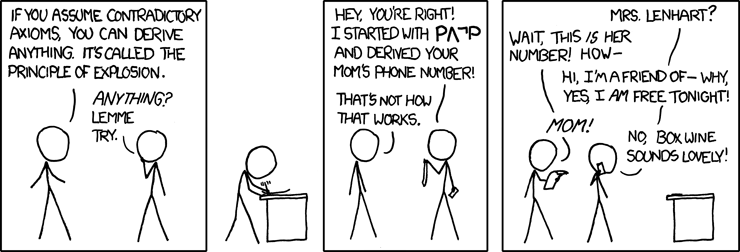
\includegraphics[width=\textwidth]{principle_of_explosion.png}

Hvis et logisk system falder sammen på sådan en måde siger vi at det er inkonsistent --
kombinationen af de modstridende aksiomer danner tilsammen en inkonsistens.
Den slags systemer er af åbentlyse grunde ret uinteressante.
Men det kan hurtigt blive svært at formulere et sæt aksiomer der beskriver komplicerede ting
og stadigvæk være sikker på at der ikke er nogen ting der strider mod hinanden.
Da man forsøgte at bygge matematikken op fra et grundlag af formel logik i slutningen
af 1800-tallet til starten af 1900-tallet stødte man flere gange ind i sådan nogen problemer,
hvor nogen nok specielt har hørt om Rusells Paradoks -- dette vil vi dog ikke komme nærmere
ind på her.

Så vi har altså to forskellige egenskaber som logiske systemer kan have: Fuldstændigt og Konsistent.
Optimalt set ville det jo være rart hvis et system er begge dele.
Men kan vi få det til at være dette? Og kan vi analysere om et system har de egenskaber?
Det første spørgsmål man kunne stille ville være hvad man ville analysere systemet med. Hvordan kan vi vide at det
vi bruger til at analysere systemet med selv er konsistent? Hvis det ikke er så ville det jo også kunne fortælle
os at systemet er inkonsistent, og så kan vi ikke rigtigt sige at være kommet frem til noget.
En ting man kunne håbe på kunne jo være at man kunne bruge et tilsyneladende simplere system til at analysere et mere komplekst system.
Selvom vi ikke ville vide det med sikkerhed kan vi måske føle os mere sikre på at et simplere system er konsistent.

Nogen systemer er så simple at vi nemt kan analysere dem. F.eks. kan vi vise at ren udsagnslogik er både fuldstændigt og konsistent.
Årsagen til dette er at man kan analysere den fulde opførsel af $\land,\lor,\imp,\neg$ og $\bimp$ ved at skrive endelige sandhedstabeller op som man
kan kontrollere værdien/korrektheden af. Lige så snart vi har med prædikatlogik at gøre kan man sådan lidt uformelt sige at vi
har introduceret et potentiale for uendelighed, så vi har ikke længere noget hvor vi kan analysere et endeligt antal muligheder.

Så kan vi så analysere prædikatlogik på en anden måde? Det kunne jo være meget rart at vide med rimelig sikkerhed om 
f.eks. \eqref{exists-is-forall} er en ufuldstændighed.

\ifdefined\startGoedel\end{document}\fi
